%%%%% This is file `elsarticle-template-1-num.tex',
%%%\documentclass[letterpaper,12pt]{article}
%%%%\documentclass[preprint,12pt]{elsarticle}
%%%
%%%%% The graphicx package provides the includegraphics command.
%%%\usepackage{graphicx}
%%%%% The amssymb package provides various useful mathematical symbols
%%%\usepackage{amssymb}
%%%%% The amsthm package provides extended theorem environments
%%%%% \usepackage{amsthm}
%%%\usepackage{lineno}
%%%\usepackage{color}
%%%\usepackage{sectsty}
%%%\subsubsectionfont{\normalfont}
%%%\subsectionfont{\normalfont}
%%%\usepackage{multirow}
%%%\usepackage{subfiles}
%%%
%%%
%%%\journal{Journal Name}

%%%\begin{document}
%%%
%%%\begin{frontmatter}
%%%
%%%%% Title, authors and addresses
%%%
%%%\title{\texttt{UQpy} - Uncertainty Quantification with Python}
%%%\author{Michael D.\ Shields, Dimitris G. Giovanis\\ Aakash Bangalore-Satish, Mohit Chauhan, Lohit Vandanapu, Jiaxin Zhang}
%%%
%%%\address{Johns Hopkins University, USA}
%%%
%%%\end{frontmatter}

%%
%% Start line numbering here if you want
%%
%%%\linenumbers
\section{Installing \texttt{UQpy}}

\underline{Prerequisites:}
You have at least one Python interpreter 3.6+ properly installed on your computer. In order to get the latest experimental version of  \texttt{UQpy} the code can be installed from Github directly as follows:

\begin{itemize}
\item[ ]  \texttt{\$git clone https://github.com/SURGroup/UQpy.git}
\item[ ] \texttt{\$cd UQpy/}
\item[ ] \texttt{\$pip install -r  requirements.txt}.
\item[ ]  \texttt{\$python setup.py install}.
\end{itemize}

\noindent
The last command might need \textbf{sudo} prefix, depending on your python setup. 

%% main text
\section{Overview}
\label{S:overview}
\noindent
\texttt{UQpy} (Uncertainty Quantification (UQ) using python) is a software toolbox containing a collection of modules  written in Python that provide standardized solutions for many UQ problems that occur in physical model. Connection between UQpy and the user-defined computational model is made with text-based and bash shell script(s) provided by the user. Execution of \texttt{UQpy} results in realizations of the parametric space of interest using advanced techniques, as well as evaluations the corresponding model responses. \texttt{UQpy} is entirely code-agnostic and gives users a fully functional tool for performing UQ with nearly any computational analysis code. \texttt{UQpy} performs submission, execution, monitoring and post-process analysis, specifically tailored to  the analysis tool and the available platform and thus, it is amenable to performing adaptive UQ methods. \texttt{UQpy} is written in the Python 3 programming language.

\subsection{Compiled version of \texttt{UQpy}}

\noindent
{\color{red} We need to address the Windows version}

\subsection{Interpreted version of \texttt{UQpy}}

\noindent
The interpreted version of \texttt{UQpy} requires a Python shell supporting Python 3.6+ as well as several common Python libraries as well.  After downloading and installing \texttt{UQpy}, the following \texttt{UQpy}-specific files are required and must be co-located in the subdirectory lib/\textbf{UQpy}, which is in the same directory as {\color{blue}UQpy\_cmd.py}:

\begin{itemize}
\item[$\cdot$] {\color{blue}UQpyModules.py} - Contains various functions.
\item[$\cdot$] {\color{blue}SampleMethods.py} - Contains the available sampling methods used for exploring the parameter space.
\item[$\cdot$] {\color{blue}ReadInputFile.py} -  Reads the necessary UQ Parameter data file  in case of running \texttt{UQpy}  via command line, and converts it to  python variables. 
\item[$\cdot$] {\color{blue}PDFs.py} - Contains the percent point functions of all the supported distributions; any new distribution can be added here. 
\end{itemize}

\section{Using UQpy- Required files}

\noindent
\texttt{UQpy} may be run using either an Integrated Development Environment (IDE) used in computer programming, specifically for the Python language or via the command line. The interpreted version of \texttt{UQpy}, has been tested to run in IDE PyCharm 2017.3.3.

In order to use  \texttt{UQpy} for evaluating the response of any computational model for a number of parameter realizations,  \texttt{UQpy}  requires three \textbf{executable}\footnote{\$\texttt{chmod +x }{\color{red}name1*.sh} } bash shell scripts: 

\begin{itemize}
\item {\color{red}name1*.sh} for linking the analysis software to \texttt{UQpy} 

\item {\color{red}name2*.sh} for converting the the file containing the parameter values (text-based file) into appropriate input file for the analysis code  

\item {\color{red}name3*.sh} converting the result of the software analysis into an appropriate  (text-based) file to be read from \texttt{UQpy}. This is necessary  in case of running adaptive UQ methods and/or post-processing of the results. 
\end{itemize}

\noindent
The names of these files are user defined. Additional to these files, if the user wants to  generate the realizations of the random parameters according to one of the  available sampling methods  provided in \texttt{UQpy}, it is necessary to provide an text-based file under the name  ({\color{magenta}UQpy\_params.txt}), which will enclose all the probabilistic information required for running the selected sampling method. T

The aforementioned files are directly specified by the user and may be in any directory.


\section{UQpy Usage}

\noindent
\texttt{UQpy} is user friendly since it only requires the user to have basic knowledge in writing bash shell scripts.

\subsection{Using the \texttt{UQpy}  Command Line Mode}

\noindent
\texttt{UQpy} can be executed directly through the command line. It is provided as an option to the user who doesn't have sufficient familiarity and experience with python. Command line execution is advantageous when analyses need to be performed on a high-performance computing systems without direct graphics capability. In order to  execute the interpreted version \texttt{UQpy} from the command line the user needs to  change to the \texttt{UQpy} directory and then type in terminal :

\vspace{4mm}
\noindent
{\scriptsize \texttt{\$python UQpy\_cmd.py --dir pathToModel --model name1*.sh --input name2*.sh --output name3*.sh}}


\vspace{4mm}
\noindent
Where

\begin{itemize}
 \item  {\color{blue} UQpy\_cmd.py} is the python script that actually runs \texttt{UQpy}  via command line and needs to be located in the directory \textbf{UQpy}.
 
 \item \texttt{--dir} is the absolute path to the folder which contains the necessary files  {\{\color{red}name1*.sh} , {\color{red}name2*.sh} , {\color{red}name3*.sh} and {\color{magenta}UQpy\_params.txt}\}.
 
 \item \texttt{--model} points to the {\color{red}name1*.sh} bash script
 
  \item \texttt{--input} points to the {\color{red}name2*.sh} bash script
  
   \item \texttt{--output} points to the {\color{red}name3*.sh} bash script
 
 \end{itemize}


\noindent
In order for \texttt{UQpy}  to run from command line  the file  {\color{magenta}UQpy\_params.txt} is necessary to be located inside \texttt{--dir} otherwise, the execution will return an error. However the user may skip the entries \{\texttt{--input, --output, --model}\}  if  \texttt{UQpy}  is utilized only for generating realizations of the random parameter and not for model evaluations.  Another optional entry for the user is \texttt{--CPUs} which sets the number of processors used for the evaluation of the model, in case of parallel processing.   The user can see all the available options (Fig. \ref{UQpy_help}) by typing in terminal

\vspace{4mm}
{\centering
	{\small \texttt{\$python UQpy\_cmd.py --help}}\par}
\vspace{4mm}


\noindent
which results in:

\begin{figure}[!ht]
	\centering	{\includegraphics[scale=0.7]{./uqpy/UQpy_help}}
	\caption{}
	\label{UQpy_help}
\end{figure}


\subsection{Using the \texttt{UQpy}  IDE Mode}
\label{sec:IDE_Mode}

\noindent
After installation, \texttt{UQpy} is build in the local Python’s standard library and thus, it runs from any Integrated Development Environment (PyCharm, Atom, Eclipse, e.t.c) which provides code analysis and debugging. In order to use \texttt{UQpy} libraries in a project the user needs to import the specific module to its workspace. This can be done by writing in a python script

\vspace{4mm}
{\centering
 \texttt{{\color{blue} from} \texttt{UQpy} {\color{blue} import} * }\par}
\vspace{4mm}

\noindent
which will load all modules of \texttt{UQpy}. If a specific class from the sample methods  (e.g Monte Carlo simulation) is required then the user can selectively load it to the project by typing 
\vspace{4mm}

{\centering
 \texttt{{\color{blue} from} \texttt{UQpy.SampleMethods} {\color{blue} import} MCS }\par}

\vspace{4mm}
\noindent
This functionality of \texttt{UQpy} enables the independent usage of its  modules, which makes \texttt{UQpy} a powerful tool for UQ analysis and communication between python and various computational codes of different nature.  In order to generate 100 realizations of two random parameters using MCS  the user needs to type:
\vspace{4mm}

{\centering
	\texttt{{\color{blue} from} \texttt{UQpy.SampleMethods} {\color{blue} import} MCS }\\
	\texttt{x = MCS(dimension=2, pdf\_type=['Uniform', 'Uniform'])\\
	pdf\_params=[[0, 1], [0, 1] ], nsamples=100)}\par}

\vspace{4mm}
\noindent
This will create the object \texttt{x} with is properties:

\begin{itemize}
	\item[1.] \texttt{pdf\_type}: type of distribution for each parameter
	\item[2.] \texttt{pdf\_params}: distribution parameters
	\item[3.] \texttt{nsamples}: number of samples to be generated
	\item[4.] \texttt{dimension}: number of random parameters
	\item[5.] \texttt{samples}: generated samples in the parameter space
	\item[6.] \texttt{samplesU01}: generated samples in the Uniform space, U[0, $1]^{\mbox{\texttt{dimension}}}$
	\end{itemize}



\section{\texttt{UQpy} workflow}


\section{Templates for the required  Files}

\noindent
The interaction between \texttt{UQpy}  and any external solver is made  with text-based files which are simple to process and easy to work with in python.  

\subsection{Probabilistic Parameter File}

\noindent
The file that keeps the probabilistic properties of the parameters should always be under the name:

\vspace{4mm}
{\centering
{\color{magenta}UQpy\_params.txt}\par}

\vspace{4mm}
\noindent
Creating {\color{magenta}UQpy\_params.txt} is simple and straightforward; Each property that is required for the selected sampling method, is defined in a line  that starts  with a hash-tag (\#),  followed by a key-word and/or key-phrase (case sensitive) describing the property\footnote{The order that the properties are declared in {\color{magenta}UQpy\_params.txt} is not important .}. The file ends with the key-word \texttt{\#end}. Under that line, the specific attributes of the property are defined, according to the \texttt{UQpy} available options. Thus, different sampling methods require different parameter file . 

\subsubsection{Required properties for various sampling methods}

The properties that need to be specified by the user inside the parameter file in order to run different sampling methods, for exploring the parameter space. A summary of these properties  is given next:  

\begin{center}
	\begin{tabular}{ |l|c|c| } 
		\hline
		\multicolumn{3}{|c|}{\textbf{Monte Carlo simulation}} \\
		\hline
		\textbf{Property} & \textbf{Mandatory} & \textbf{Optional} \\
		\hline
		 \texttt{\#method}& $\star$ &   \\ 
		\hline
		\texttt{\#number of samples}& $\star$ &   \\ 
		\hline
		\texttt{\#number of parameters}& $\star$  &   \\ 
		\hline
		\texttt{\#distribution type}& $\star$ &   \\ 
		\hline
		\texttt{\#distribution parameters} & $\star$ &   \\ 
		\hline
		\texttt{\#names of parameters}& & $\star$   \\ 
		\hline
		\texttt{\#SROM}&  & \textbf{True} or \textbf{False}  \\ 
		\hline
	\end{tabular}
\end{center}

\begin{center}
	\begin{tabular}{ |l|c|c| } 
				\hline
		\multicolumn{3}{|c|}{\textbf{Latin hypercube simulation}} \\
		\hline
		\textbf{Property} & \textbf{Mandatory} & \textbf{Optional} \\
		\hline
		\texttt{\#method}& $\star$ &   \\ 
		\hline
		\texttt{\#number of samples}& $\star$ &   \\ 
		\hline
		\texttt{\#number of parameters}&  $\star$  &   \\ 
		\hline
		\texttt{\#distribution type}& $\star$ &   \\ 
		\hline
		\texttt{\#distribution parameters} & $\star$ &   \\ 
		\hline
		\texttt{\#names of parameters}& & $\star$   \\ 
		\hline
		\texttt{\#criterion}& & $\star$   \\ 
		\hline
		\texttt{\#distance}& & $\star$   \\ 
		\hline
		\texttt{\#metric}& & $\star$   \\ 
		\hline
				\texttt{\#SROM}&  & \textbf{True} or \textbf{False}    \\ 
		\hline
	\end{tabular}
\end{center}

\begin{center}
	\begin{tabular}{ |l|c|c| } 
		\hline
		\multicolumn{3}{|c|}{\textbf{Stratified sampling}} \\
		\hline
		\textbf{Property} & \textbf{Mandatory} & \textbf{Optional} \\
		\hline
		\texttt{\#method}& $\star$ &   \\ 
		\hline
		\texttt{\#distribution type}& $\star$ &   \\ 
		\hline
		\texttt{\#number of parameters}& &$\star$    \\ 
		\hline
		\texttt{\#distribution parameters} & $\star$ &   \\ 
		\hline
		\texttt{\#design}& $\star$ &    \\ 
		\hline
		\texttt{\#names of parameters}& & $\star$   \\ 
		\hline
				\texttt{\#SROM}&  & \textbf{True} or \textbf{False}    \\ 
		\hline
	\end{tabular}
\end{center}

\begin{center}
	\begin{tabular}{ |l|c|c| } 
		\hline
		\multicolumn{3}{|c|}{\textbf{Partially Stratified sampling}} \\
		\hline
		\textbf{Property} & \textbf{Mandatory} & \textbf{Optional} \\
		\hline
		\texttt{\#method}& $\star$ &   \\ 
		\hline
		\texttt{\#distribution type}& $\star$ &   \\ 
		\hline
		\texttt{\#distribution parameters} & $\star$ &   \\ 
		\hline
		\texttt{\#number of parameters}& &$\star$    \\ 
		\hline
		\texttt{\#design}& $\star$  &  \\ 
		\hline
		\texttt{\#strata}& $\star$ &   \\ 
		\hline
		\texttt{\#names of parameters}& & $\star$   \\ 
		\hline
				\texttt{\#SROM}&  & \textbf{True} or \textbf{False}    \\ 
		\hline
	\end{tabular}
\end{center}




\begin{center}
	\begin{tabular}{ |l|c|c| } 
		\hline
		\multicolumn{3}{|c|}{\textbf{Stochastic reduced order model}} \\
		\hline
		\textbf{Property} & \textbf{Mandatory} & \textbf{Optional} \\
		\hline
		\multicolumn{3}{|c|}{If \texttt{\#SROM} property is \textbf{True}} \\
		\hline
		\texttt{\#moments}& $\star$ &   \\ 
		\hline
		\texttt{\#error function weights} & $\star$ &   \\ 
		\hline
		\texttt{\#properties to match}&  &  $\star$  \\ 
		\hline
		\texttt{\#sample weights}& & $\star$   \\ 
		\hline
	\end{tabular}
\end{center}


\subsubsection{Examples of parameter files}


\noindent
 Special instruction on how to create the parameter file that will enclose the required properties of the selected sampling method are the following :
 
 \begin{itemize}
 	 	\item  A complete parameter file for  e.g. Monte Carlo simulation can defined like Fig.\ref{template_mcs}(a).
 	
 	\item  If all random parameters follow the same distribution type with the same distribution parameters then a parameter file  can defined like Fig.\ref{template_mcs}(b) where the distribution type and parameters need to be defined once. In this case existence of the property  "number of random parameters" is mandatory.
 	
 	 \item  For the case the number of distribution type is equal to the number of distribution parameters (Fig.\ref{template_mcs}(c))  then, definition of property "number of parameters" is optional .
 	\end{itemize}


\begin{figure}[!ht]
	\centering	{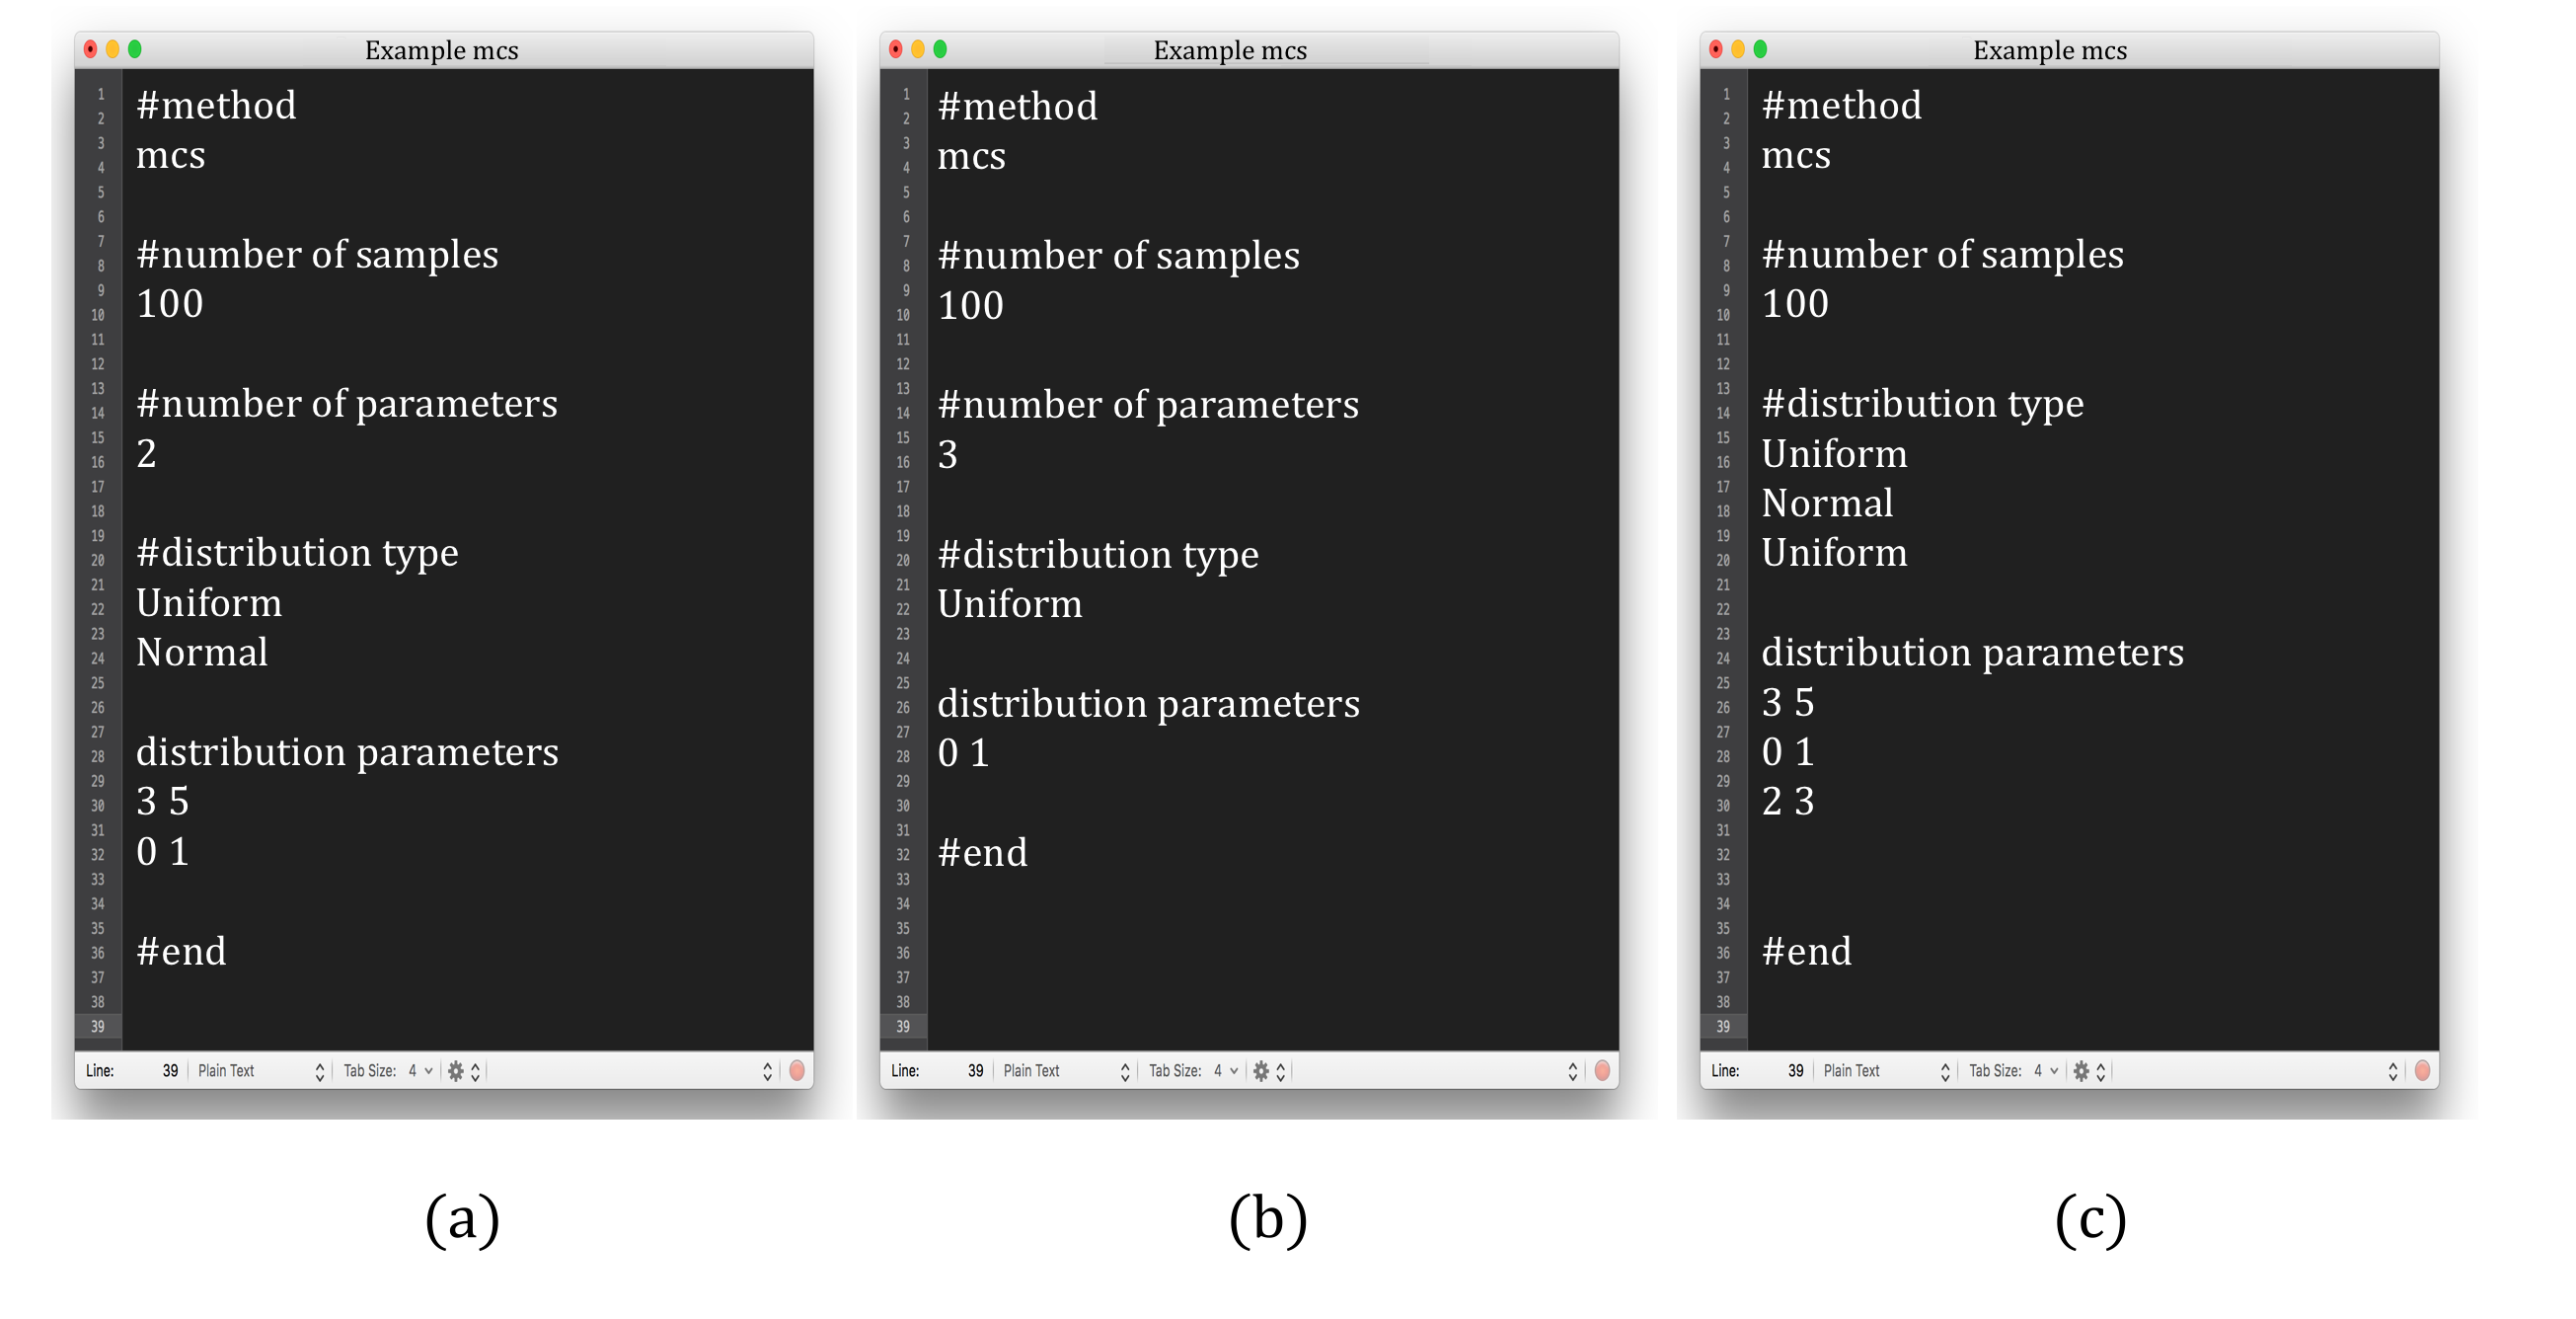
\includegraphics[scale=0.3]{./uqpy/template_mcs}}
	\caption{}
	\label{template_mcs}
\end{figure}



\subsection{Template Input File}

The functionality of the {\color{red} name2*.sh} bash shell script file is to convert the text-based output file of \texttt{UQpy}   ({\color{magenta} UQpy\_run\_i.txt}) that contains the realization {\color{magenta} i}  of the parameter vector into appropriate input  for the analysis code.  The user is responsible for creating the appropriate bash script for performing this action. For example, if the software code reads a text-based  file called {\color{magenta} modelInput\_i.txt} then a possible {\color{red} name2*.sh} script would be the one depicted in Fig.\ref{template_input};  it is used for renaming {\color{magenta} UQpy\_run\_i.txt } to {\color{magenta} modelInput\_i.txt}.


\begin{figure}[!ht]
	\centering	{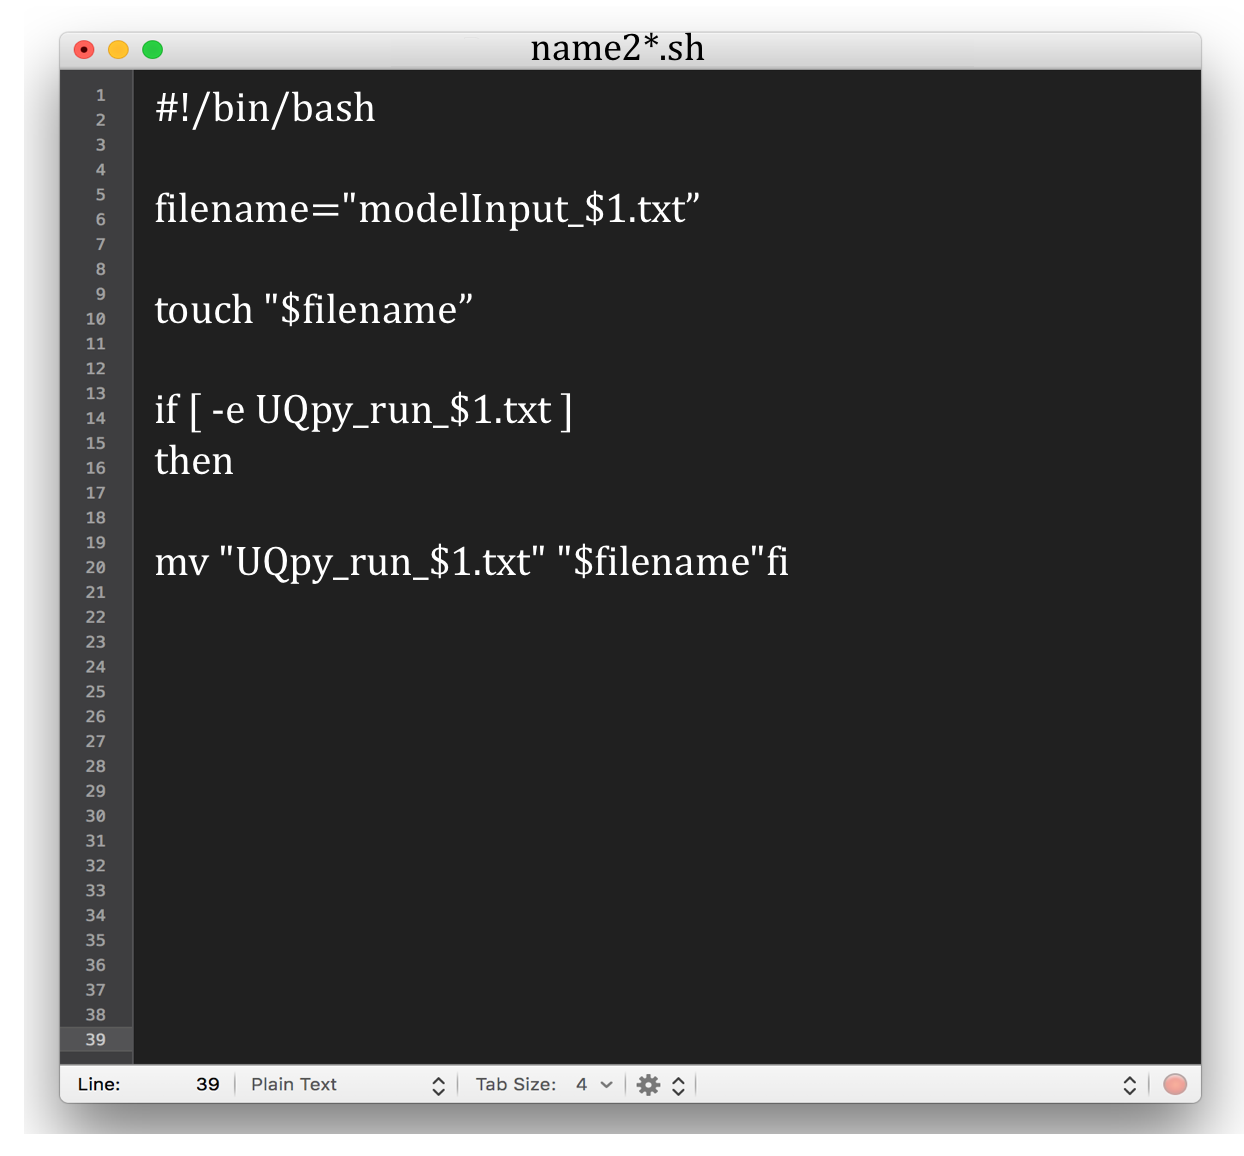
\includegraphics[scale=0.40]{template_input}}
	\caption{}
	\label{template_input}
\end{figure}



\subsection{Template Model File}

In order for \texttt{UQpy}  to execute the software code a bash script ({\color{red} name1*.sh} ) is necessary.  


\begin{figure}[!ht]
	\centering	{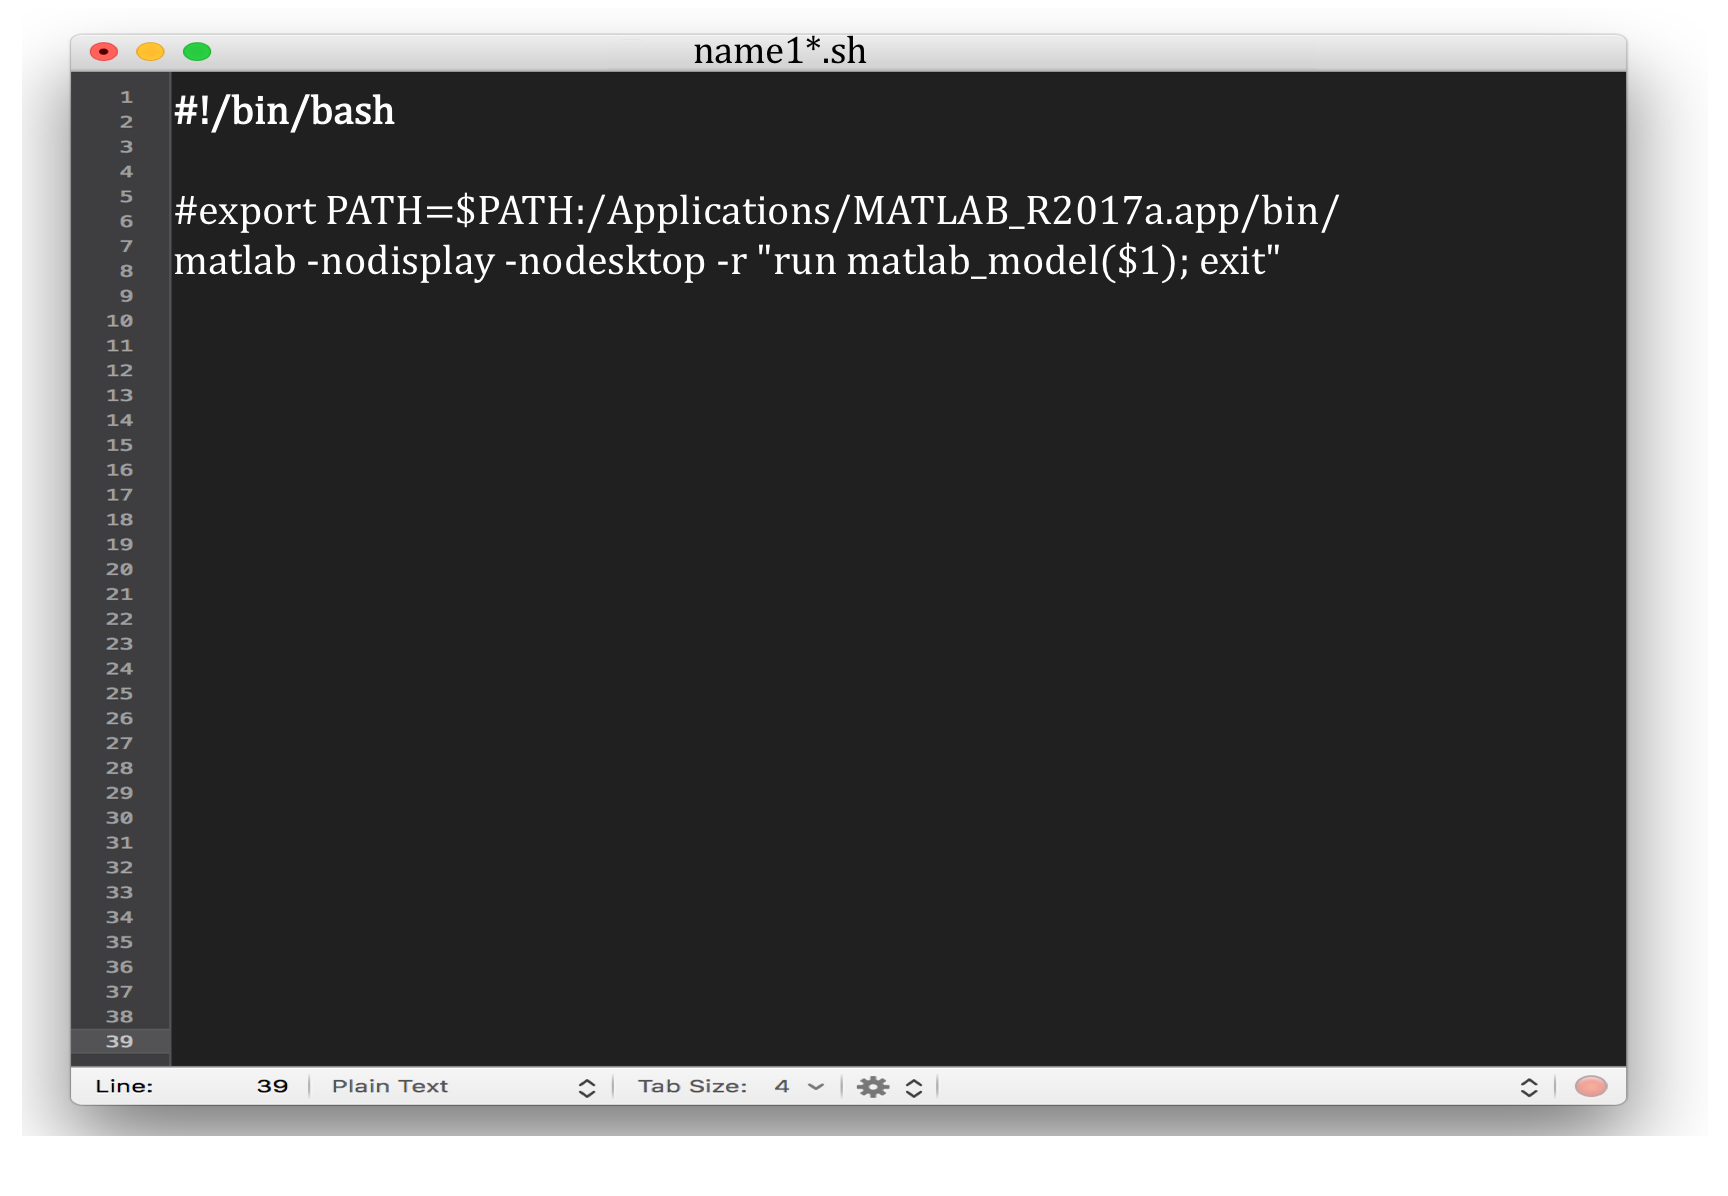
\includegraphics[scale=0.40]{template_model}}
	\caption{}
	\label{template_model}
\end{figure}



\subsection{Template Output File}

The functionality of the {\color{red} name3*.sh} bash shell script file is to convert the output of the code analysis (which can be at any format) into a text file file under the name {\color{magenta} UQpy\_eval\_i.txt"}, where {\color{magenta} i} refers to the number of simulation,  ready to be processed by \texttt{UQpy}. This step is required for running adaptive UQ methods as well as for post-processing of the result but in any case it is mandatory to provide such file. For example, if the software code generates a text-based  file called {\color{magenta} solution\_i.txt} then a possible {\color{red} name3*.sh} script would be the one depicted in Fig.\ref{template_output};  it is used for renaming {\color{magenta} solution\_i.txt} to {\color{magenta} UQpy\_eval\_i.txt"}.


\begin{figure}[!ht]
	\centering	{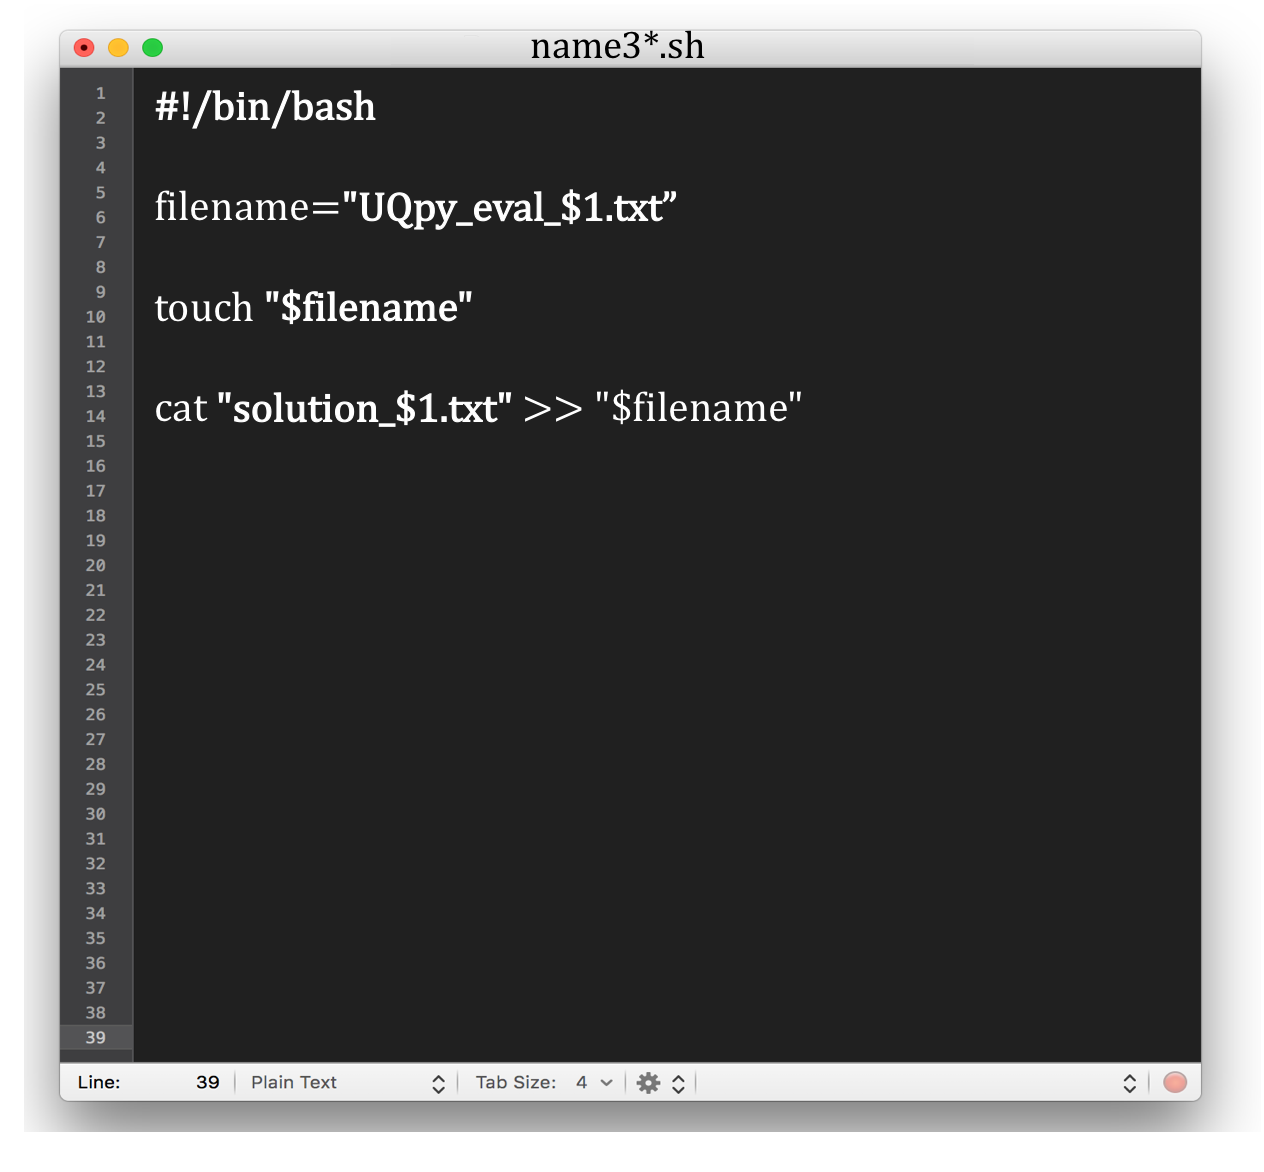
\includegraphics[scale=0.40]{template_output}}
	\caption{}
	\label{template_output}
\end{figure}

%\subfile{./uqpy/Modules}

\section{\texttt{UQpy} Modules, Classes, \& Functions}

\texttt{UQpy} is structured in five core modules, each centered around specific functionalities:
\begin{enumerate}
\item \texttt{SampleMethods}: This module contains a set of classes and functions to draw samples from random variables. These samples may be randomly drawn, as in Monte Carlo simulation, or they may be deterministically drawn as in stochastic collocation or quasi-Monte Carlo.
\item \texttt{Inference}: This module contains a set of classes and functions to conduct probabilistic inference. The module contains methods that are based on Bayesian, frequentist, likelihood, and information theories. 
\item \texttt{Reliability}: This module contains a set of classes and functions designed specifically to estimate probability of failure.
\item \texttt{Surrogate}: This module contains a set of classes and functions for building surrogate models, meta-models, or emulators.
\item \texttt{Sensitivity}: This module contains a set of classes and functions for performing global and local sensitivity analysis.
\item \texttt{RunModel}: This module contains a set of classes and functions that allows \texttt{UQpy} to initiate simulations using either python or third-party computational solvers.
\end{enumerate}
The following sections detail the classes and functions in each module with reference to examples that illustrate their use. Guidance is based on usage in IDE Model (see Section \ref{sec:IDE_Mode})

%%%%%%%%%%%%%%%%%%%%%%%%%%%%%%%%%%%%%%%%%%%%%%%%%%%%%%%%%%%
%																						%
% 									SampleMethods Module									%
%																						%
%%%%%%%%%%%%%%%%%%%%%%%%%%%%%%%%%%%%%%%%%%%%%%%%%%%%%%%%%%%

\subsection{\texttt{SampleMethods} Module}

The \texttt{SampleMethods} module consists of classes and functions to draw samples from random variables. It is imported in a python script using the following command:

\vspace{4mm}
\texttt{{\color{blue} from} \texttt{UQpy} {\color{blue} import} SampleMethods }
\vspace{4mm}

\noindent
The \texttt{SampleMethods} module has the following classes, each corresponding to a different sampling method:

\vspace{4mm}
\begin{center}
	\begin{tabular}{ |l|l| } 
		\hline
		\textbf{Class} &  \textbf{Method} \\
		\hline
		\texttt{MCS}&  Monte Carlo Sampling  \\ 
		\hline
		\texttt{LHS}&  Latin Hypercube Sampling  \\ 
		\hline
		\texttt{STS}&  Stratified Sampling  \\ 
		\hline
		\texttt{PSS}&  Partially Stratified Sampling  \\ 
		\hline
		\texttt{MCMC}&  Markov Chain Monte Carlo  \\ 
		\hline
		\texttt{SROM}&  Stochastic Reduced Order Model  \\ 
		\hline
	\end{tabular}
\end{center}
\vspace{4mm}

\noindent
Each class can be imported individually into a python script. For example, the MCMC class can be imported to a script using the following command:

\vspace{4mm}
\texttt{{\color{blue} from} \texttt{UQpy.SampleMethods} {\color{blue} import} MCMC}
\vspace{4mm}

\noindent
The following subsections describe each class, their respective inputs and attributes, and their use.

%%%%%%%%%%%%%%%%%%%%%%%%%%%%%%%%%%%%%%%%%%%%%%%%%%%%%%%%%%%
% Monte Carlo sampling

\subsubsection{\texttt{UQpy.SampleMethods.MCS}}

%%%%%%%%%%%%%%%%%%%%%%%%%%%%%%%%%%%%%%%%%%%%%%%%%%%%%%%%%%%
% Latin hypercube sampling

\subsubsection{\texttt{UQpy.SampleMethods.LHS}}

\begin{center}
	\begin{tabular}{ |l|c|l| } 
		\hline
		\textbf{Property} & \textbf{Type} & \textbf{Options} \\
		\hline
		\texttt{\#criterion}& \textit{string} &  'random', 'centered', 'maximin', 'correlate'  \\ 
		\hline
		\multirow{5}{*}{\texttt{\#distance}} & \multirow{5}{*}{\textit{string}} & 'braycurtis', 'canberra', 'chebyshev', 'cosine', \\ 
		&  &  'dice', 'euclidean', 'hamming', 'jaccard',  'cityblock',   \\ 
		&  &  'matching', 'minkowski', 'rogerstanimoto',  'correlation', \\ 
		&  & 'sokalmichener', 'sokalsneath', 'sqeuclidean',  \\ 
		&  & ' 'kulsinski', 'mahalanobis', 'russellrao', 'seuclidean',  \\ 
		\hline
	\end{tabular}
\end{center}

%%%%%%%%%%%%%%%%%%%%%%%%%%%%%%%%%%%%%%%%%%%%%%%%%%%%%%%%%%%
% Stratified Sampling

\subsubsection{\texttt{UQpy.SampleMethods.STS}}

%%%%%%%%%%%%%%%%%%%%%%%%%%%%%%%%%%%%%%%%%%%%%%%%%%%%%%%%%%%
% Partially Stratified Sampling

\subsubsection{\texttt{UQpy.SampleMethods.PSS}}

%%%%%%%%%%%%%%%%%%%%%%%%%%%%%%%%%%%%%%%%%%%%%%%%%%%%%%%%%%%
% MCMC

\subsubsection{\texttt{UQpy.SampleMethods.MCMC}}
\label{Sec:MCMC}

The \texttt{MCMC} class is imported using the following command:

\vspace{4mm}
\texttt{{\color{blue} from} \texttt{UQpy.SampleMethods} {\color{blue} import} MCMC}
\vspace{4mm}

\noindent
The attributes of the \texttt{MCMC} class are listed below:

\begin{center}
%	\resizebox{\textwidth}{!}{
	\begin{tabular}{ |l|c|c|c| } 
				\hline
		\multicolumn{4}{|c|}{\texttt{MCMC} Class Attribute Definitions} \\
		\hline
		\textbf{Attribute} & \textbf{Input/Output} & \textbf{Required} & \textbf{Optional} \\
		\hline
		\texttt{dimension} & Input &  & $\star$  \\ 
		\hline
		\texttt{pdf\_proposal\_type} & Input & & $\star$   \\ 
		\hline
		\texttt{pdf\_proposal\_scale} & Input &  & $\star$  \\ 
		\hline
		\texttt{pdf\_target\_type}& Input &  &  $\star$  \\ 
		\hline
		\texttt{pdf\_target} & Input & $\star$ &   \\ 
		\hline
		\texttt{pdf\_target\_params} & Input  & &  $\star$  \\ 
		\hline
		\texttt{algorithm} & Input &  & $\star$  \\ 
		\hline
		\texttt{jump} & Input &  & $\star$  \\ 
		\hline
		\texttt{nsamples}& Input & $\star$ &    \\ 
		\hline
		\texttt{seed} & Input & & $\star$   \\ 
		\hline
		\texttt{nburn} & Input & & $\star$   \\ 
		\hline
		\texttt{samples} & Output & & \\
		\hline
	\end{tabular}%}
\end{center}

\noindent
A brief description of each attribute can be found in the table below:

\begin{center}
	\resizebox{\textwidth}{!}{
	\begin{tabular}{ |l|c|c|c| } 
				\hline
		\multicolumn{4}{|c|}{\texttt{MCMC} Class Attributes} \\
		\hline
		\textbf{Attribute} & \textbf{Type} & \textbf{Options} & \textbf{Default} \\
		\hline
		\texttt{dimension} & {\it integer} &  & \texttt{dimension} = 1  \\ 
		\hline
		\texttt{algorithm} & {\it string} & \begin{tabular}[t]{c}`MH'\\`MMH'\\`Stretch' \end{tabular} & `MMH'  \\ 
		\hline
		\texttt{pdf\_proposal\_type} & {\it string} & \begin{tabular}[t]{c}`Normal'\\`Uniform' \end{tabular}& `Uniform'   \\ 
		\hline
		\texttt{pdf\_proposal\_scale} & \begin{tabular}[t]{c}{\it float}\\{\it float list} \end{tabular} &  & \begin{tabular}[t]{c}if \texttt{algorithm} = `MMH' or `MH': \\ \texttt{pdf\_proposal\_scale} ={[1,1,\dots,1]}\\ if \texttt{algorithm}=`Stretch':\\ \texttt{pdf\_proposal\_scale} = 2 \end{tabular}  \\ 
		\hline
		\texttt{pdf\_target\_type}& {\it string} & \begin{tabular}[t]{c}`marginal\_pdf'\\`joint\_pdf' \end{tabular} &  \begin{tabular}[t]{c}if \texttt{algorithm} = `MMH': \\ \texttt{pdf\_target\_type} = `marginal\_pdf'\\ if \texttt{algorithm}=`Stretch':\\ \texttt{pdf\_target\_type} = `joint\_pdf' \end{tabular}  \\ 
		\hline
		\texttt{pdf\_target} & \begin{tabular}[t]{c}{\it function}\\{\it string} \end{tabular} &  & Normal($\mathbf{0},\mathbf{I}$)  \\ 
		\hline
		\texttt{pdf\_target\_params} & \begin{tabular}[t]{c}{\it float}\\{\it float list} \end{tabular}  & &  \texttt{None} \\ 
		\hline
		\texttt{jump} & {\it integer} &  & 1  \\ 
		\hline
		\texttt{nsamples}& {\it integer} &  & \texttt{None}   \\ 
		\hline
		\texttt{seed} & \begin{tabular}[t]{c}{\it nparray}\\{\it nparray list} \end{tabular} & & \begin{tabular}[t]{c}array(0,0,\dots,0)\\size = $1\times \texttt{dimension}$ \end{tabular}    \\ 
		\hline
		\texttt{nburn} & {\it integer} & & 0   \\ 
		\hline
		\texttt{samples} & {\it nparray} & & \\
		\hline
	\end{tabular}}
\end{center}

\noindent\textbf{Detailed Description of \texttt{MCMC} Class Attributes:}\\

\noindent\textit{Input Attributes}:
\begin{itemize}
\item \texttt{dimension}:\\ 
	A scalar integer value defining the dimension of the random variables. 
\item \texttt{algorithm}: \\ 
	Specifies the algorithm used to generate samples. \texttt{UQpy} currently supports three commonly used algorithms.
	\begin{itemize}
		\item `MH': \\ 
			Metropolis-Hastings algorithm. For a description of the algorithm, see \cite{Metropolis1953,Hastings1970,Au2001}. 
		\item `MMH': \\ 
			Component-wise modified Metropolis-Hastings algorithm. For a description of the algorithm, see \cite{Au2001}. 
		\item `Stretch': \\ 
			Affine invariant ensemble sampler employing ``stretch" moves. For a description of the algorithm, see \cite{Goodman2010}.
	\end{itemize} 
\item \texttt{pdf\_proposal\_type}:\\ 
	Type of proposal density function. This option is only invoked when \texttt{algorithm} = `MH' or `MMH'. \texttt{UQpy} currently supports two types of proposal densities:
	\begin{itemize}
		\item `Normal': \\
			The proposal density is specified as a normal distribution with mean value equal to the current state of the Markov Chain and standard deviation specified by 						\texttt{pdf\_proposal\_scale}. That is, a new candidate sample is generated as\\ $x_{i+1}\sim N(x_i,\texttt{pdf\_proposal\_scale})$.
		\item `Uniform': \\
			The proposal density is specified as a uniform distribution with centered at the current state of the Markov Chain with width equal to \texttt{pdf\_proposal\_scale}. That is, a 			new candidate sample is generated as\\ $x_{i+1}\sim U(x_i-\texttt{pdf\_proposal\_scale}/2,x_i+\texttt{pdf\_proposal\_scale}/2)$.
		\end{itemize}
		When $\texttt{dimension}>1$, \texttt{pdf\_proposal\_type} may be specified as a string or a list of strings assigned to each dimension. When \texttt{pdf\_proposal\_type} is 			specified as a string, the same proposal type is specified for all dimensions.
\item \texttt{pdf\_proposal\_scale}:\\ 
	Sets the scale of the proposal probability density. The scale of the proposal density depends on both the MCMC algorithm employed (\texttt{algorithm}) and the type of proposal 		density specified (\texttt{pdf\_proposal\_type}).
	\begin{itemize}
		\item For \texttt{algorithm} = `MH' or `MMH', this defines either the standard deviation of a normal proposal density or the width of a uniform density. See 							\texttt{pdf\_proposal\_type} above.
		\item For \texttt{algorithm} = `Stretch', this sets the scale of the stretch density $g(z)=\frac{1}{\sqrt{z}},\sim z\in[1/\texttt{pdf\_proposal\_scale}, \texttt{pdf\_proposal\_scale}]$. See 		\cite{Goodman2010}.
	\end{itemize}
	When $\texttt{dimension}>1$, \texttt{pdf\_proposal\_scale} may be specified as a scalar or a list of values assigned to each dimension. When \texttt{pdf\_proposal\_scale} is specified 	as a scalar, the same scale is specified for all dimensions. 
\item \texttt{pdf\_target\_type}: 

	[Use only with \texttt{algorithm} = `MMH']\\ 
	
	MCMC algorithms use acceptance-rejection based on a ratio of the target probability densities between the current state and the proposed state. In the `MH' algorithm and the 		`Stretch' algorithm, the ratio of probabilities is computed using the target joint pdf. For the `MMH' algorithm with independent random variables, acceptance/rejection can be computed 	based on the ratio of the marginals for each dimension. This variable specifies whether to use a ratio of target joint pdf's or a ratio of target marginal pdf's in the acceptance-rejection 	step for each dimension of the `MMH' algorithm. This option is not used for the `MH' and `Stretch' algorithms.
	\begin{itemize}
		\item `joint\_pdf': \\
			Compute the acceptance-rejection using the ratio of the target joint pdf's. [Always use when random variables are dependent.]
		\item `marginal\_pdf': \\
			Compute the acceptance-rejection using the ratio of target marginal pdf's in each dimension. [Only use when random variables are independent.]
	\end{itemize} 
\item \texttt{pdf\_target}:\\ 
	Specifies the target probability density function from which to draw MCMC samples (i.e.\ the stationary distribution of the Markov chain). \texttt{pdf\_target} must be passed into 		\texttt{MCMC} as a function. In \texttt{UQpy}, this can be achieved in two ways:
	\begin{itemize}
		\item Direct function definition:\\
		The easiest way to define \texttt{pdf\_target} is to create a function in the python script that calls \texttt{MCMC}. When the function is directly defined, \texttt{pdf\_target} is 			specified directly using the function name (not as a string). 
		\item Definition through `custom\_pdf.py':\\
		If the function is to be called frequently by the user or may need to be shared among python scripts in a project, the user may define the function in a python script 					`custom\_pdf.py' that resides in the user's working directory. When this is the case, \texttt{pdf\_target} is specified by a string that corresponds to the function name in 				`custom\_pdf.py'. See Section \ref{Sec:Distributions} for a detailed description of `custom\_pdf.py'.
	\end{itemize} 
	In both cases, the function must be defined to accept two parameters: 
	\begin{enumerate}
		\item The point at which to compute the pdf, 
		\item A list of parameters of the pdf specified through \texttt{pdf\_target\_params} 
	\end{enumerate}
	If the pdf does not have any user-defined parameters, the user still must define the function to accept a parameter list.\\

	When $\texttt{dimension}>1$ and \texttt{pdf\_target\_type} = `marginal\_pdf', \texttt{pdf\_target} may be specified as a string/function or a list of strings/functions assigned to each 		dimension. When specified as a string/function, the same marginal pdf is specified for all dimensions.
\item \texttt{pdf\_target\_params}:\\
	Parameters of the target pdf to be passed into the function defined by \texttt{pdf\_target}.
\item \texttt{jump}\\
	Specifies the number of samples between accepted states of the Markov chain. Setting \texttt{jump} = 1 corresponds to accepting every state. Setting $\texttt{jump} = n$ corresponds 	skipping $n-1$ states between accepted states of the chain.
\item \texttt{nsamples}\\
	Specifies the number of samples to be generated (not including skipped states of the chain). \texttt{nsamples} must be specified. There is no default value.
\item \texttt{seed}\\
	Specifies the initial state of the Markov chain. \\
	
	For \texttt{algorithm} = `MMH' or `MH', this is a numpy array of zeros with size $1\times \texttt{dimension}$.\\
	
	For \texttt{algorithm} = `Stretch', this is a list of $n_s$ points, each defined as numpy arrays with size $1\times \texttt{dimension}$, where $n_s$ is the size of the ensemble being 		propagated. \cite{Goodman2010}. The default value in the table above is not valid for  \texttt{algorithm} = `Stretch'.
\item \texttt{nburn}\\
	Specifies the number of samples at the start of the chain to be discarded as ``burn-in." This option is only applicable for \texttt{algorithm}=`MMH' and `MH'
\end{itemize}

\noindent\textit{Output Attributes}:
\begin{itemize}
\item \texttt{samples}:\\
	The only output of the \texttt{MCMC} class are the generated samples. The samples are returned as a numpy array of dimension $\texttt{nsamples}\times\texttt{dimension}$. 
\end{itemize}

\noindent\textbf{Examples:}\\
\noindent Two examples illustrating the use of the \texttt{MCMC} class are provided in the following Jupyter scripts.
\begin{itemize}
\item MCMC\_Example1.ipynb:\\
	In this example, the three MCMC algorithms are used to generate 1000 samples from a two-dimensional Rosenbrock pdf. The Rosenbrock pdf is defined as a function directly in the 	script.
\item MCMC\_Example2.ipynb:\\
	In this example, the three MCMC algorithms are used to generate 1000 samples from a two-dimensional Rosenbrock pdf. The Rosenbrock pdf is defined as a function in the 			`custom\_pdf.py' script.
\end{itemize}

%\begin{center}
%	\begin{tabular}{ |l|c|l| } 
%		\hline
%		\textbf{Property} & \textbf{Type} & \textbf{Description/Options} \\
%		\hline
%		\texttt{\#criterion}& \textit{string} &  'random', 'centered', 'maximin', 'correlate'  \\ 
%		\hline
%		\multirow{5}{*}{\texttt{\#distance}} & \multirow{5}{*}{\textit{string}} & 'braycurtis', 'canberra', 'chebyshev', 'cosine', \\ 
%		&  &  'dice', 'euclidean', 'hamming', 'jaccard',  'cityblock',   \\ 
%		&  &  'matching', 'minkowski', 'rogerstanimoto',  'correlation', \\ 
%		&  & 'sokalmichener', 'sokalsneath', 'sqeuclidean',  \\ 
%		&  & ' 'kulsinski', 'mahalanobis', 'russellrao', 'seuclidean',  \\ 
%		\hline
%	\end{tabular}
%\end{center}
%
%
%\begin{center}
%	\begin{tabular}{ |l|l| } 
%		\hline
%		\textbf{Property} &  \textbf{Options} \\
%		\hline
%		\texttt{\#target distribution}&   'multivariate\_pdf', 'marginal\_pdf', 'normal\_pdf'  \\ 
%		\hline
%		\texttt{\#proposal distribution}&   'Uniform', 'Normal'  \\ 
%		\hline
%		\texttt{\#algorithm}&   'MH', 'MMH'  \\ 
%		\hline
%	\end{tabular}
%\end{center}

%%%%%%%%%%%%%%%%%%%%%%%%%%%%%%%%%%%%%%%%%%%%%%%%%%%%%%%%%%%
% SROM




\subsubsection{Adding a sampling method in \texttt{UQpy}}

%%%%%%%%%%%%%%%%%%%%%%%%%%%%%%%%%%%%%%%%%%%%%%%%%%%%%%%%%%%
%																						%
% 									Inference Module										%
%																						%
%%%%%%%%%%%%%%%%%%%%%%%%%%%%%%%%%%%%%%%%%%%%%%%%%%%%%%%%%%%

\subsection{\texttt{Inference} Module}

Coming soon\dots

%%%%%%%%%%%%%%%%%%%%%%%%%%%%%%%%%%%%%%%%%%%%%%%%%%%%%%%%%%%
%																						%
% 									Reliability Module										%
%																						%
%%%%%%%%%%%%%%%%%%%%%%%%%%%%%%%%%%%%%%%%%%%%%%%%%%%%%%%%%%%

\subsection{\texttt{Reliability} Module}

The \texttt{Reliability} module consists of classes and functions to provide simulation-based estimates of probability of failure from a given user-defined computational model and failure criterion. It is imported in a python script using the following command:

\vspace{4mm}
\texttt{{\color{blue} from} \texttt{UQpy} {\color{blue} import} Reliability }
\vspace{4mm}

\noindent
The \texttt{Reliability} module has the following classes, each corresponding to a method for probability of failure estimation:

\vspace{4mm}
\begin{center}
	\begin{tabular}{ |l|l| } 
		\hline
		\textbf{Class} &  \textbf{Method} \\
		\hline
		\texttt{SubsetSimulation}&  Subset Simulation  \\ 
		\hline
		\texttt{FORM}&  First Order Reliability Method  \\ 
		\hline
		\texttt{SORM}& Second Order Reliability Method  \\ 
		\hline
	\end{tabular}
\end{center}
\vspace{4mm}

\noindent
Each class can be imported individually into a python script. For example, the \texttt{SubsetSimulation} class can be imported to a script using the following command:

\vspace{4mm}
\texttt{{\color{blue} from} \texttt{UQpy.SampleMethods} {\color{blue} import} SubsetSimulation}
\vspace{4mm}

\noindent
The following subsections describe each class, their respective inputs and attributes, and their use.

%%%%%%%%%%%%%%%%%%%%%%%%%%%%%%%%%%%%%%%%%%%%%%%%%%%%%%%%%%%
% Subset Simulation

\subsubsection{\texttt{UQpy.Reliability.SubsetSimulation}}


The \texttt{SubsetSimulation} class is imported using the following command:

\vspace{4mm}
\texttt{{\color{blue} from} \texttt{UQpy.Reliability} {\color{blue} import} SubsetSimulation}
\vspace{4mm}

\noindent
The attributes of the \texttt{SubsetSimulation} class are listed below:

\begin{center}
%	\resizebox{\textwidth}{!}{
	\begin{tabular}{ |l|c|c|c| } 
				\hline
		\multicolumn{4}{|c|}{\texttt{SubsetSimulation} Class Attribute Definitions} \\
		\hline
		\textbf{Attribute} & \textbf{Input/Output} & \textbf{Required} & \textbf{Optional} \\
		\hline
		\texttt{dimension} & Input &  & $\star$  \\ 
		\hline
        \texttt{nsamples\_init}& Input &  &  $\star$  \\ 
		\hline
        \texttt{nsamples\_ss}& Input & $\star$ &    \\ 
		\hline
        \texttt{p\_cond}& Input &  &  $\star$  \\ 
		\hline
        \texttt{algorithm} & Input &  & $\star$  \\ 
		\hline
		\texttt{pdf\_target\_type}& Input &  &  $\star$  \\ 
		\hline
		\texttt{pdf\_target} & Input & $\star$ &   \\ 
		\hline
		\texttt{pdf\_target\_params} & Input  & &  $\star$  \\ 
		\hline
		\texttt{pdf\_proposal\_type} & Input & & $\star$   \\ 
		\hline
		\texttt{pdf\_proposal\_scale} & Input &  & $\star$  \\ 
		\hline
		\texttt{model\_type}& Input &  &   $\star$ \\ 
		\hline
		\texttt{model\_script}& Input & $\star$ &    \\ 
		\hline
		\texttt{input\_script}& Input &  & $\star$   \\ 
		\hline
		\texttt{output\_script}& Input &  & $\star$   \\ 
		\hline
		\texttt{samples} & Output & & \\
		\hline
		\texttt{g} & Output & & \\
		\hline
		\texttt{g\_level} & Output & & \\
		\hline
		\texttt{pf} & Output & & \\
		\hline
	\end{tabular}%}
\end{center}


\noindent
A brief description of each attribute can be found in the table below:

\begin{center}
	\resizebox{\textwidth}{!}{
	\begin{tabular}{ |l|c|c|c| } 
				\hline
		\multicolumn{4}{|c|}{\texttt{SubsetSimulation} Class Attributes} \\
		\hline
		\textbf{Attribute} & \textbf{Type} & \textbf{Options} & \textbf{Default} \\
		\hline
		\texttt{dimension} & {\it integer} &  & \texttt{dimension} = 1  \\ 
		\hline
        \texttt{samples\_init} & {\it nparray} &  & \texttt{None}  \\ 
		\hline
        \texttt{nsamples\_ss}& {\it integer} &  & \texttt{None}   \\ 
		\hline
        \texttt{p\_cond} & {\it float} & $0<\texttt{p\_cond}<1$ & $\texttt{p\_cond}=0.1$  \\ 
		\hline
        \texttt{algorithm} & {\it string} & \begin{tabular}[t]{c}`MMH'\\`Stretch' \end{tabular} & `MMH'  \\ 
		\hline
		\texttt{pdf\_target\_type}& {\it string} & \begin{tabular}[t]{c}`marginal\_pdf'\\`joint\_pdf' \end{tabular} &  `marginal\_pdf'  \\ 
		\hline
		\texttt{pdf\_target} & \begin{tabular}[t]{c}{\it function}\\{\it string} \end{tabular} &  & Normal($\mathbf{0},\mathbf{I}$)  \\ 
		\hline
		\texttt{pdf\_target\_params} & \begin{tabular}[t]{c}{\it float}\\{\it float list} \end{tabular}  & &  \texttt{None} \\ 
		\hline
		\texttt{pdf\_proposal\_type} & {\it string} & \begin{tabular}[t]{c}`Normal'\\`Uniform' \end{tabular}& `Uniform'   \\ 
		\hline
		\texttt{pdf\_proposal\_scale} & \begin{tabular}[t]{c}{\it float}\\{\it float list} \end{tabular} &  & \begin{tabular}[t]{c}\texttt{algorithm} = `MMH' or `MH' \\ {[1,1,\dots,1]}\\ \texttt{algorithm}=`Stretch'\\ 2 \end{tabular}  \\ 
		\hline
		\texttt{model\_type} & {\it string} & See \texttt{UQpy.RunModel} & See \texttt{UQpy.RunModel}  \\ 
		\hline
		\texttt{model\_script} & {\it string} & See \texttt{UQpy.RunModel} & See \texttt{UQpy.RunModel}  \\ 
		\hline
		\texttt{input\_script} & {\it string} & See \texttt{UQpy.RunModel} & See \texttt{UQpy.RunModel}  \\ 
		\hline
		\texttt{output\_script} & {\it string} & See \texttt{UQpy.RunModel} & See \texttt{UQpy.RunModel}  \\ 
		\hline
		\texttt{samples} & {\it nparray list} & & \\
		\hline
		\texttt{g} & {\it nparray list} & &   \\ 
		\hline
		\texttt{g\_level} & {\it list} & &    \\ 
		\hline
		\texttt{pf} & {\it float} & &   \\ 
		\hline
	\end{tabular}}
\end{center}


\noindent\textbf{Detailed Description of \texttt{SubsetSimulation} Class Attributes:}\\

\noindent\textit{Input Attributes}:
\begin{itemize}
\item \texttt{dimension}:\\ 
	A scalar integer value defining the dimension of the random variables. 
\item \texttt{samples\_init}\\
	Specifies the initial samples for subset/level 0. The size of the array \texttt{samples\_init} must be \texttt{nsamples\_ss}$\times$\texttt{dimension}. These samples can be generated in any way the user chooses.\\
    
    If \texttt{samples\_init} is not specified, the subset/level 0 samples are drawn internally in \texttt{SubsetSimulation} using the component-wise Modified Metropolis-Hastings algorithm.
\item \texttt{nsamples\_ss}\\
	Specifies the number of samples to be generated in each conditional level (i.e.\ per subset). \texttt{nsamples\_ss} must be specified. There is no default value.
\item \texttt{p\_cond}\\
	Specifies the conditional probability for each subset.\\
    
    The current implementation does not allow for variable conditional probabilities (i.e.\ setting different conditional probabilities for each level).\\
    
    The current implementation does not allow for the conditional probabilities to be defined implicitly by instead specifying the intermediate failure domains explicitly.
\item \texttt{algorithm}: \\ 
	Specifies the MCMC algorithm used to generate samples in each conditional level. \texttt{SubsetSimulation} currently supports two commonly-used algorithms.
	\begin{itemize}
		\item `MMH': \\ 
			Component-wise modified Metropolis-Hastings algorithm. For a description of the algorithm, see \cite{Au2001}. 
		\item `Stretch': \\ 
			Affine invariant ensemble sampler employing ``stretch" moves. For a description of the algorithm, see \cite{Goodman2010}.
	\end{itemize} 
    \texttt{SubsetSimulation} currently does not support the conventional Metropolis-Hastings algorithm.
\item \texttt{pdf\_target\_type}:\\ 
	This is used for Markov Chain Monte Carlo (MCMC) sampling from the conditional probability densities in subset simulation. For details, the user is referred to documentation for 		\texttt{UQpy.SampleMethods.MCMC} in Section \ref{Sec:MCMC}
\item \texttt{pdf\_target}:\\ 
	This is used for Markov Chain Monte Carlo (MCMC) sampling from the conditional probability densities in subset simulation. For details, the user is referred to documentation for 		\texttt{UQpy.SampleMethods.MCMC} in Section \ref{Sec:MCMC}
\item \texttt{pdf\_target\_params}:\\
	This is used for Markov Chain Monte Carlo (MCMC) sampling from the conditional probability densities in subset simulation. For details, the user is referred to documentation for 		\texttt{UQpy.SampleMethods.MCMC} in Section \ref{Sec:MCMC}
\item \texttt{pdf\_proposal\_type}:\\ 
	This is used for Markov Chain Monte Carlo (MCMC) sampling from the conditional probability densities in subset simulation. For details, the user is referred to documentation for 		\texttt{UQpy.SampleMethods.MCMC} in Section \ref{Sec:MCMC}
\item \texttt{pdf\_proposal\_scale}:\\ 
	This is used for Markov Chain Monte Carlo (MCMC) sampling from the conditional probability densities in subset simulation. For details, the user is referred to documentation for 		\texttt{UQpy.SampleMethods.MCMC} in Section \ref{Sec:MCMC}
\item \texttt{model\_type}\\
	This is used to evaluate the model at each sample point using the \texttt{RunModel} class. For details, the user is referred to documentation for \texttt{UQpy.RunModel} in Section \ref{Sec:RunModel}.
\item \texttt{model\_script}\\
	This is used to evaluate the model at each sample point using the \texttt{RunModel} class. For details, the user is referred to documentation for \texttt{UQpy.RunModel} in Section \ref{Sec:RunModel}.\\
    
    Note that a computational model must be specified using \texttt{model\_script}. Without this model, \texttt{SubsetSimulation} cannot run.
\item \texttt{input\_script}\\
	This is used to evaluate the model at each sample point using the \texttt{RunModel} class. For details, the user is referred to documentation for \texttt{UQpy.RunModel} in Section \ref{Sec:RunModel}.
\item \texttt{output\_script}\\
	This is used to evaluate the model at each sample point using the \texttt{RunModel} class. For details, the user is referred to documentation for \texttt{UQpy.RunModel} in Section \ref{Sec:RunModel}.
\end{itemize}

\noindent\textit{Output Attributes}:
\begin{itemize}
\item \texttt{samples}:\\
	Contains the sample values from each conditional level as a list of numpy arrays.\\
    
    Each item of the list is a numpy array containing the samples from the corresponding conditional level. For example, \texttt{SubsetSimulation.samples[0]} contains a numpy array of dimension \texttt{nsamples\_ss}$\times$\texttt{dimension} with the samples from conditional level 0 (i.e.\ the initial sample set).
\item \texttt{g}\\
	Returns the scalar values of the performance function evaluated by the computational model at each point in \texttt{samples}. \texttt{g} is structured in the same manner as \texttt{samples} (a {\it numpy array list}) with each entry equal to the performance function evaluation of the corresponding sample.\\
    
    By convention, failure of a given sample \texttt{sample[i][j]} is defined by $\texttt{g[i][j]}<0$, where \texttt{i} indexes the conditional level and \texttt{j} indexes the sample number. For use with \texttt{SubsetSimulation}, the user's computational model must return a scalar value that follows this convention. The value is passed from \texttt{RunModel} into \texttt{SubsetSimulation} through the attribute \texttt{RunModel.model\_eval.QOI} as detailed in Section \ref{Sec:RunModel}.
\item \texttt{g\_level}\\
	Specifies the value of the performance function for each conditional level. \texttt{g\_level} is structured as a list with each entry of the list equal to the value of the corresponding performance function at the respective conditional level. For example, \texttt{g\_level[3]} corresponds to the performance function value that defines the third subset.
    
    Note that \texttt{g\_level} is implicitly defined by the samples and \texttt{p\_cond}. \texttt{UQpy} currently does not support the direct assignment of conditional performance levels.
\item \texttt{pf}\\
	Probability of failure estimate from subset simulation
\end{itemize}

\noindent\textbf{\texttt{SubsetSimulation} Examples:}\\
\noindent Two examples illustrating the use of the \texttt{MCMC} class are provided in the following Jupyter scripts.
\begin{itemize}
\item MCMC\_Example1.ipynb:\\
	In this example, the three MCMC algorithms are used to generate 1000 samples from a two-dimensional Rosenbrock pdf. The Rosenbrock pdf is defined as a function directly in the 	script.
\item MCMC\_Example2.ipynb:\\
	In this example, the three MCMC algorithms are used to generate 1000 samples from a two-dimensional Rosenbrock pdf. The Rosenbrock pdf is defined as a function in the 			`custom\_pdf.py' script.
\end{itemize}


%%%%%%%%%%%%%%%%%%%%%%%%%%%%%%%%%%%%%%%%%%%%%%%%%%%%%%%%%%%
% FORM

\subsubsection{\texttt{UQpy.Reliability.FORM}}

Coming soon\dots

%%%%%%%%%%%%%%%%%%%%%%%%%%%%%%%%%%%%%%%%%%%%%%%%%%%%%%%%%%%
% SORM

\subsubsection{\texttt{UQpy.Reliability.SORM}}

Coming soon\dots

%%%%%%%%%%%%%%%%%%%%%%%%%%%%%%%%%%%%%%%%%%%%%%%%%%%%%%%%%%%
%																						%
% 									Surrogate Module										%
%																						%
%%%%%%%%%%%%%%%%%%%%%%%%%%%%%%%%%%%%%%%%%%%%%%%%%%%%%%%%%%%

\subsection{\texttt{Surrogate} Module}


\subsubsection{\texttt{UQpy.Surrogates.SROM}}

The \texttt{SROM} class is imported using the following command:

\vspace{4mm}
\texttt{{\color{blue} from} \texttt{UQpy.Surrogates} {\color{blue} import} SROM}
\vspace{4mm}

\noindent
The attributes of the \texttt{SROM} class are listed below:

\begin{center}
%	\resizebox{\textwidth}{!}{
	\begin{tabular}{ |l|c|c|c| } 
				\hline
		\multicolumn{4}{|c|}{\texttt{SROM} Class Attribute Definitions} \\
		\hline
		\textbf{Attribute} & \textbf{Input/Output} & \textbf{Required} & \textbf{Optional} \\
		\hline
		\texttt{samples} & Input & $\star$ &   \\ 
		\hline
        \texttt{pdf\_type}& Input & $\star$ &    \\ 
		\hline
        \texttt{pdf\_params}& Input & $\star$ &    \\ 
		\hline
        \texttt{moments}& Input & $\star$ &    \\ 
		\hline
        \texttt{correlation} & Input & & $\star$   \\ 
		\hline
        \texttt{weights\_error} & Input &  & $\star$  \\ 
		\hline
		\texttt{weights\_distribution}& Input &  &  $\star$  \\ 
		\hline
		\texttt{weights\_moments} & Input &  &  $\star$ \\ 
		\hline
		\texttt{weights\_correlation} & Input  & &  $\star$  \\ 
		\hline
        \texttt{properties} & Input & & $\star$   \\ 
		\hline
		\texttt{sample\_weights} & Output &  &   \\ 
		\hline
	\end{tabular}%}
\end{center}


\noindent
A brief description of each attribute can be found in the table below:

\begin{center}
	\resizebox{\textwidth}{!}{
	\begin{tabular}{ |l|c|c|c| } 
				\hline
		\multicolumn{4}{|c|}{\texttt{SROM} Class Attributes} \\
		\hline
		\textbf{Attribute} & \textbf{Type} & \textbf{Options} & \textbf{Default} \\
		\hline
		\texttt{samples} & \begin{tabular}[t]{c}{\it ndarray}\\{\it list} \end{tabular} &  & \texttt{None} \\ 
		\hline
        \texttt{pdf\_type} & \begin{tabular}[t]{c}{\it function}\\{\it string} \end{tabular} &  & \texttt{None}  \\ 
		\hline
        \texttt{pdf\_params}& \begin{tabular}[t]{c}{\it ndarray}\\{\it list} \end{tabular} &  & \texttt{None}   \\ 
		\hline
        \texttt{moments} & \begin{tabular}[t]{c}{\it float ndarray}\\{\it float list} \end{tabular} &  & \texttt{None}  \\ 
		\hline
        \texttt{correlation} & \begin{tabular}[t]{c}{\it ndarray}\\{\it list}  \end{tabular} & & Identity matrix \\ 
		\hline
        \texttt{weights\_error} & {\it list} &  & [1, 0.2, 0]  \\ 
		\hline
		\texttt{weights\_distribution}& \begin{tabular}[t]{c}{\it ndarray}\\{\it list}  \end{tabular} &  &    \\ 
		\hline
		\texttt{weights\_moments} & \begin{tabular}[t]{c}{\it ndarray}\\{\it list}  \end{tabular} &  &  \\ 
		\hline
		\texttt{weights\_correlation} & \begin{tabular}[t]{c}{\it ndarray}\\{\it list}  \end{tabular}  & &  \\ 
		\hline
        \texttt{properties} & {\it boolean list} & & [`True',`True',`True',`False'] \\ 
		\hline
		\texttt{sample\_weights} & {\it ndarray} & & \\
		\hline
	\end{tabular}}
\end{center}

\noindent\textbf{Detailed Description of \texttt{SROM} Class Attributes:}\\

\noindent\textit{Input Attributes}:
\begin{itemize}
\item \texttt{samples}:\\ 
An array or list containing the samples for Stochastic Reduced Order Model. Size of array should be $nsamples \times dimension$. 

\item \texttt{pdf\_type}:\\ 
A list of functions or strings specifying Cumulative Distribution Function (CDF) of random variables.\\ \\
When $\texttt{dimension}>1$, \texttt{pdf\_type} may be specified as a string/function or a list of strings/functions assigned to each dimension. When specified as a string/function, the same cdf is specified for all dimensions.

\item \texttt{pdf\_params}:\\ 
A list of parameters corresponding to each random variable. \\ \\
When $\texttt{dimension}=1$, pdf\_params[0] should contain all the parameters. \\
For $\texttt{dimension} \geq 1$ and $\texttt{pdf\_type} = [`Gamma']$, pdf\_params should be $[[2,1,3]]$ , where random variables have gamma distribution with shape, shift and scale parameters equal to 2, 1 and 3.

\item \texttt{moments}:\\ 
A list or array specifying first and second order moment about origin corresponding to each random variable. \\ \\
It is defined such that size of array is $2 \times \texttt{dimension}$, where first row/element contains first order moment and second row/element contains second order moment.

\item \texttt{correlation}:\\ 
A list or array specifying correlation among random variables. It is defined such that size of array is $\texttt{dimension} \times \texttt{dimension}$.

\item \texttt{weights\_error}:\\
SROM generates \texttt{sample\_weights}, which optimize error between distribution, moments and correlation of samples and model.   \texttt{weights\_error} are weights corresponding to each property in objective function. It is a list of size 3.

\item \texttt{weights\_distribution}:\\
A list or array of weights corresponding to error in distribution at each sample of random variables. SROM class support following options for \texttt{weights\_distribution}:
	\begin{itemize}
    	\item {`None'}:
        Default value is defined as array of size same as \texttt{samples} with each value equal to 1.
        \item {Array of size $1 \times \texttt{dimension}$}:
        Equal weights are assigned to all samples in same dimension.
        \item {Array of size same as \texttt{samples}}
    \end{itemize}
    
\item \texttt{weights\_moments}:\\
A list or array of weights corresponding to error in moments in each dimension. SROM class support following options for \texttt{weights\_moments}:
\begin{itemize}
    	\item {`None'}:
        Default value is defined as array of size same as \texttt{moments} with each value equal to reciprocal of square of moments.
        \item {Array of size $1 \times \texttt{dimension}$}:
        Equal weights are assigned to both moments in same dimension.
        \item {Array of size same as \texttt{moments}}
    \end{itemize}
    
\item \texttt{weights\_correlation}:\\
A list or array of weights corresponding to error in correlation among random variables. It is define such that size of array is same as \texttt{correlation}.

\item \texttt{properties}:\\
A boolean list containing information about properties which are included in objective function. SROM class reduces error between distribution, first order moment about origin, second order moment about origin and correlation. Therefore, size of the list is 4. `True' includes corresponding property in objection function and `False' doesn't include it.
\end{itemize}

\noindent\textit{Output Attributes}:
\begin{itemize}

\item {\texttt{sample\_weights}}: \\
An array of reduced order weights corresponding to \texttt{samples}.

\end{itemize}
%%%%%%%%%%%%%%%%%%%%%%%%%%%%%%%%%%%%%%%%%%%%%%%%%%%%%%%%%%%
%																						%
% 									Sensitivity Module										%
%																						%
%%%%%%%%%%%%%%%%%%%%%%%%%%%%%%%%%%%%%%%%%%%%%%%%%%%%%%%%%%%

\subsection{\texttt{Sensitivity} Module}

Coming soon\dots


%%%%%%%%%%%%%%%%%%%%%%%%%%%%%%%%%%%%%%%%%%%%%%%%%%%%%%%%%%%
%																						%
% 									RunModel Module										%
%																						%
%%%%%%%%%%%%%%%%%%%%%%%%%%%%%%%%%%%%%%%%%%%%%%%%%%%%%%%%%%%

\subsection{\texttt{RunModel} Module}
\label{Sec:RunModel}

The \texttt{RunModel} module is how \texttt{UQpy} calls user-defined computational models and collects the results from the output of those simulations. Using the \texttt{RunModel} module requires the user to be familiar with either shell scripting or python scripting.  The \texttt{RunModel} module consists of a single class, also called \texttt{RunModel}, that can be imported using the following command:

\vspace{4mm}
\texttt{{\color{blue} from} \texttt{UQpy.RunModel} {\color{blue} import} RunModel}
\vspace{4mm}

\noindent
The attributes of the \texttt{RunModel} class are listed below:

\begin{center}
%	\resizebox{\textwidth}{!}{
	\begin{tabular}{ |l|c|c|c| } 
				\hline
		\multicolumn{4}{|c|}{\texttt{RunModel} Class Attribute Definitions} \\
		\hline
		\textbf{Attribute} & \textbf{Input/Output} & \textbf{Required} & \textbf{Optional} \\
		\hline
		\texttt{dimension} & Input &  & $\star$  \\ 
		\hline
        \texttt{samples}& Input &  &  $\star$  \\ 
		\hline
		\texttt{model\_type}& Input &  &   $\star$ \\ 
		\hline
		\texttt{model\_script}& Input & $\star$ &    \\ 
		\hline
		\texttt{input\_script}& Input &  & $\star$   \\ 
		\hline
		\texttt{output\_script}& Input &  & $\star$   \\ 
		\hline
		\texttt{model\_eval} & Output & & \\
		\hline
	\end{tabular}%}
\end{center}

\noindent
A brief description of each attribute can be found in the table below:

\begin{center}
	\resizebox{\textwidth}{!}{
	\begin{tabular}{ |l|c|c|c| } 
				\hline
		\multicolumn{4}{|c|}{\texttt{SubsetSimulation} Class Attributes} \\
		\hline
		\textbf{Attribute} & \textbf{Type} & \textbf{Options} & \textbf{Default} \\
		\hline
		\texttt{dimension} & {\it integer} &  & \texttt{dimension} = 1  \\ 
		\hline
        \texttt{samples} & {\it nparray} &  & \texttt{None}  \\ 
		\hline
		\texttt{model\_type} & {\it string} & \begin{tabular}[t]{c} `python' \\ \texttt{None}  \end{tabular} & \texttt{None}  \\ 
		\hline
		\texttt{model\_script} & {\it string} & Must be `.py' or `.sh' &   \\ 
		\hline
		\texttt{input\_script} & {\it string} & Must be `.py' or `.sh' &   \\ 
		\hline
		\texttt{output\_script} & {\it string} & Must be `.py' or `.sh' &   \\ 
		\hline
		\texttt{model\_eval} & {\it class object} & \begin{tabular}[t]{c} \texttt{RunPythonModel} \\ \texttt{RunSerial} \\ \texttt{RunParallel}  \end{tabular} &   \\ 
		\hline
	\end{tabular}}
\end{center}

\noindent There are two general workflows for the \texttt{RunModel} class. In the first, a model is defined or called through python scripts, which allows all message passing to be performed internally  and therefore has less computational ``overhead." In the second workflow, information is passed between \texttt{UQpy} and a third-party solver through text files. The following sections detail these two workflows.

\subsubsection{\texttt{RunModel} with direct Python communications (\texttt{model\_type} = `python')}

The fastest, simplest, and preferred way to run a model using \texttt{UQpy} is by linking \texttt{UQpy} to a Python script that calls or runs the model. This link occurs by calling the \texttt{RunModel} class, setting \texttt{model\_type} = `python', and pointing it to the user-defined Python script that will execute the model. \texttt{RunModel} is pointed to the Python script by defining the input parameter \texttt{model\_script} as a string having the name of the Python script (note this file must be a .py file). More details on defining \texttt{model\_script} can be found in Section \ref{sec:RM_attributes}. Figure \ref{fig:RunModel_Python} shows a general flow-chart for the \texttt{RunModel} class.
\begin{figure}[!ht]
	\centering	{\includegraphics[width=0.5\textwidth]{RunModel_Python}}
	\caption{General workflow for running a model from a python script (\texttt{model\_type} = `pthon') using the \texttt{RunModel} class of \texttt{UQpy}.}
	\label{fig:RunModel_Python}
\end{figure}

\texttt{UQpy} calls the Python script defined by \texttt{model\_script} through the class \texttt{RunPythonModel}, which must be present in \texttt{model\_script} and defined as follows:

\vspace{4mm}
\texttt{{\color{blue} class} \texttt{RunPythonModel:}}\\

\hspace{1cm} \texttt{def \_\_init\_\_(self, samples=None, dimension=None):}\\

\hspace{1cm} \texttt{self.samples = samples}

\hspace{1cm} \texttt{self.dimension = dimension}

\hspace{1cm} \texttt{self.QOI = list()}
\vspace{4mm}

\noindent The \texttt{RunPythonModel} class in \texttt{model\_script} must accept, as input, a set of samples and the dimension of the samples and return, as output, a list containing the quantity of interest (\texttt{self.QOI}) computed for each sample. The attributes of the \texttt{RunPythonModel} are described below. Beyond these minimal requirements, the user has complete freedom to perform whatever operations she/he desires. That is, \texttt{model\_script} may be used directly to perform some operations on the samples (e.g. solve a set of differential equations having parameters defined by the samples) or to call a third-party model (e.g.\ Matlab, Abaqus, or a custom simulation code). 


\begin{center}
%	\resizebox{\textwidth}{!}{
	\begin{tabular}{ |l|c|l| } 
				\hline
		\multicolumn{3}{|c|}{\texttt{RunPythonModel} Class Attributes} \\
		\hline
		\textbf{Attribute} & \textbf{Type} & \textbf{Description}  \\
		\hline
		\texttt{dimension} & {\it integer} & Dimension of the samples array. \\ 
		\hline
		\texttt{samples} & {\it nparray} & Sample points at which to evaluate the model. \\ 
		\hline
		\texttt{QOI} & {\it nparray} & A list containing the quantity of interest returned from the model. Each item of the list corresponds to an associated sample value and may be of arbitrary data type.  \\ 
		\hline
	\end{tabular}%}
\end{center}

\noindent\textbf{Examples:}\\
\noindent An example illustrating the use of the \texttt{RunModel} class with \texttt{model\_type} = `python' is provided in the following Jupyter script.
\begin{itemize}
\item Run\_Python\_Model.ipynb:\\
	In this example, the component-wise modified Metropolis-Hasting algorithm for MCMC is used to generate 15 (approximately) independent samples from a two-dimensional Rosenbrock pdf. The Rosenbrock pdf is defined as a function directly in the script. The samples are then passed to a Python model that evaluates the sum of the components of each sample and returns the sum as the quantity of interest (\texttt{x.model\_eval.QOI}).
\end{itemize}

Running a model in Python is strongly preferred both from the perspective of flexibility for the user, but also because it alleviates the burden of file passing as a means of communication between \texttt{UQpy} and model input/output. This is the topic of the next section.

\subsubsection{\texttt{RunModel} with file passing communications (\texttt{model\_type = None})}
The \texttt{RunModel} class supports an alternate means of running a model for users who prefer shell scripting or who prefer a more prescriptive workflow. This alternate means of running uses a set of scripts and text files to pass information from \texttt{UQpy} to a third-party model. This method of running the model supports both serial computation and parallel processing across multiple cores. It does not currently support distributed processing across multiple nodes in an HPC. 

\begin{figure}[!ht]
	\centering	{\includegraphics[width=\textwidth]{RunModel}}
	\caption{}
	\label{template_model}
\end{figure}

\begin{figure}[!ht]
	\centering	{\includegraphics[width=0.5\textwidth]{input_script}}
	\caption{}
	\label{template_model}
\end{figure}


\begin{figure}[!ht]
	\centering	{\includegraphics[width=0.5\textwidth]{model_script}}
	\caption{Need to edit this to include the model running on a computer}
	\label{template_model}
\end{figure}

\begin{figure}[!ht]
	\centering	{\includegraphics[width=0.5\textwidth]{output_script}}
	\caption{}
	\label{template_model}
\end{figure}

\subsubsection{Calling \texttt{RunModel} and defining its attributes}
\label{sec:RM_attributes}

\subsubsection{Necessary files and scripts}

\subsection{Supporting Modules, Functions, and Files}

\subsubsection{\texttt{Distributions} Module}
\label{Sec:Distributions}

The \texttt{Distributions} module is a support module that performs probability distribution related operations.  This includes functions for computing probabilities densities, cumulative distributions, and their inverses for common distribution types. 

The \texttt{Distributions} module is imported in a Python script using the following command:

\vspace{4mm}
\texttt{{\color{blue} from} \texttt{UQpy} {\color{blue} import} Distributions}
\vspace{4mm}

The \texttt{Distributions} module contains the following functions:

\vspace{4mm}
\begin{center}
	\begin{tabular}{ |l|l| } 
		\hline
		\textbf{Function} &  \textbf{Operation} \\
		\hline
		\texttt{pdf}& Probability Density Function  \\ 
		\hline
	\end{tabular}
\end{center}
\vspace{4mm}

The input and output of the \texttt{pdf} function are described in the table below.

\begin{center}
%	\resizebox{\textwidth}{!}{
	\begin{tabular}{ |l|c|c|c| } 
				\hline
		\multicolumn{4}{|c|}{\texttt{pdf} Function I/O} \\
		\hline
		\textbf{Attribute}  & Input/Output & \textbf{Type} & \textbf{Options} \\
		\hline
		\texttt{dist} & Input & {\it string} & Custom \\ 
		\hline
		\texttt{return} & Output & {\it float} & N/A \\ 
		\hline
	\end{tabular}%}
\end{center}

\noindent The \texttt{pdf} function enables the evaluation of a standard pdf or an arbitrary user-defined probability density function. When a custom pdf is used, the pdf is defined through the Python script `custom\_pdf.py', which must be located in the current working directory. Details follow.\\

\noindent\textbf{Description of \texttt{custom\_pdf.py}}\\

\noindent The script `custom\_pdf.py' allows the user to define a custom probability density function. In the script, the user may define a function that computes the pdf at a specified sample point. The function definition follows standard Python scripting conventions. For compatibility with \texttt{UQpy}, each function must be defined as follows:

\vspace{4mm}
\texttt{{\color{blue} def} func\_name(x, params)}\\
\hspace*{1.3cm} \texttt{pdf\_value = [User-defined operations]}\\
\hspace*{1.3cm} \texttt{return pdf\_value}
\vspace{4mm}

\noindent The name of the function, \texttt{func\_name}, can be specified arbitrarily by the user but must be identical to the name provided as a {\it string} to the value of \texttt{dist} from the \texttt{pdf} function described above.\\

\noindent The function is required to take two inputs: 
\begin{itemize}
\item \texttt{x}: (type = {\it float})\\ 
	The sample value at which to evaluate the probability density function.
\item \texttt{params}: (type = {\it list})\\
	A list of parameters for the probability density function. If the function does not require any parameters, the function must still take \texttt{params} as input. The user may then pass an 	empty list.
\end{itemize}

\noindent The function returns only the value of the pdf evaluate at \texttt{x}, defined by \texttt{pdf\_value}.\\

\noindent An example `custom\_pdf.py' file is provided with the second example from the \texttt{MCMC} class, MCMC\_Example2.ipynb. See Examples from Section \ref{Sec:MCMC}.


%%%\section*{References}
%%%
%%%\bibliographystyle{model1-num-names}
%%%\bibliography{UQpy_bib}
%%%
%%%\end{document}

%%
%% End of file `elsarticle-template-1-num.tex'.
